\section{Inherent Gamma of camera and projectors}

Gamma is an inherent property of digital imaging systems \cite{Wang2014}. It is defined by the following equation:
\begin{equation}
V_{out} = {V_{in}}^\gamma
\end{equation}
where $V_{out}$ is the output luminance value $V_{in}$ is the actual luminance value of each pixel in an image, and $\gamma$ is the gamma factor of the imaging system \cite{McHugh2014}. The gamma factor changes the appearance of a digital image as it reaches our eyes. Once the image is saved (JPG, TIFF, etc.), compression happens and gamma is already encoded in it \cite{Wang2014}.

A better explanation of gamma encoding is illustrated in Figure \ref{fig:gammafactor}. The original gradient is a 5-bit (32 levels) image which was encoded linearly and with gamma. The differences between the three are clearly observed in the manner of spacing of the gray levels. 

\captionsetup[figure]{width=5in}
\begin{figure}[h!]
	\centering
	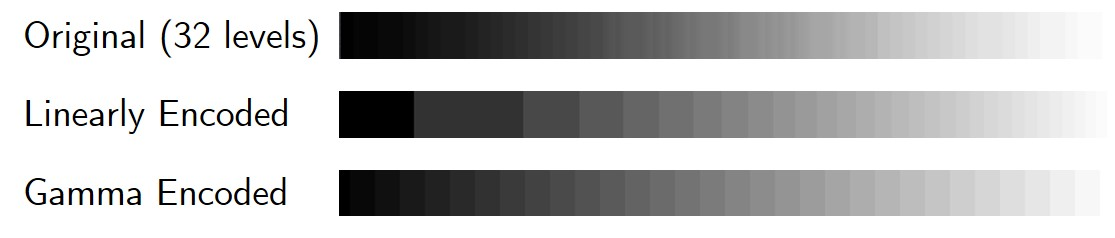
\includegraphics[width=0.75\textwidth]{figures/gammafactor.jpg}
	\caption[Grayscale 5-bit gradients]{A grayscale 5-bit gradient (top). The linearly encoded image (middle) has lesser dark tones and more lighter tones, and the gamma endoded (bottom) has evenly-spaced gray levels \cite{McHugh2014}.}
	\label{fig:gammafactor}
\end{figure}

LCD projectors also do gamma encoding by displaying images with adjusted pixel intensities for more detailed and enhanced projected images \cite{Li2011}. 

In a PSP setup, inherent gamma of both projector and camera combines and is encoded in the output images producing a nonlinear input-output curve. Corrections must then be done to remove the distortion introduced by gamma.
